\documentclass{exam}

\usepackage{units} 
\usepackage{xfrac} 
\usepackage[fleqn]{amsmath}
\usepackage{cancel}
\usepackage{float}
\usepackage{mdwlist}
\usepackage{booktabs}
\usepackage{cancel}
\usepackage{polynom}
\usepackage{caption}
\usepackage{fullpage}
\usepackage{comment}
\usepackage{enumerate}
\usepackage{graphicx}
\usepackage{parskip}

\everymath{\displaystyle}

\printanswers

\ifprintanswers 
  \usepackage{2in1, lscape} 
\fi

\title{Statistics \\ Homework Five}
\date{\today}
\author{}

\begin{document}

  \maketitle

  \section{Homework}
    \begin{itemize*}
      \item read Chapter 5 
      \item take a look at the ``Check Your Skills'' exercises
      \item exercises: 
    \end{itemize*}

  \ifprintanswers
    \begin{description}

      \item[27]     
        \begin{figure}[H]
          \centering
          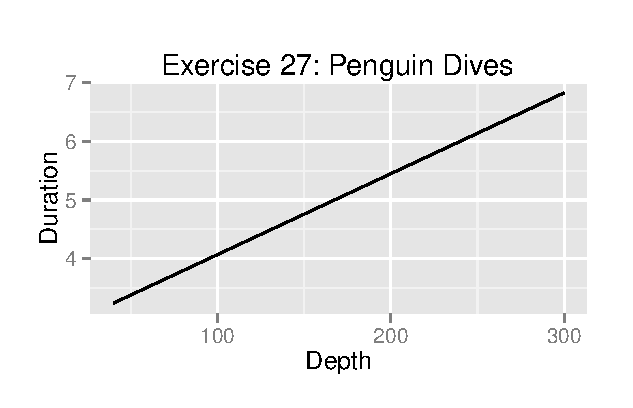
\includegraphics{figures/ex27.eps}
          \caption{Exercise 27}
        \end{figure}

        \begin{parts}
          \part $m = \unit[0.0138]{m/s}$  Every 0.0138 meters of dive depth takes the
          penguin another second of dive time.

        \part 
          \[
            DD(200) = 2.69 + 0.0138 \cdot 200 \approx \unit[5.45]{s}
          \]
        \end{parts}
    
      \item[28]
        \begin{parts}
          \part for every $\unit[1.507]{mg/l}$ increase in the concentration of TOC,
            there is a $\unit[1]{mg/l}$ increase in the concentration of BOD.

          \part The predicted value is $\unit[-55.43]{mg/l}$.  Perhaps nothing can
            live when the total organic carbon is close to zero, so the BOD value
            doesn't make sense.
        \end{parts}
    \end{description}


  \else
    \vspace{10 cm}
    \begin{quote}
      \begin{em}
        The more corrupt a society, the more numerous its laws.
      \end{em}
    \end{quote}
    \hspace{1 cm} --Edward Abbey
  \fi

\end{document}

